\documentclass{exam}
%\documentclass[11pt,a4paper]{exam}
\usepackage{amsmath,amsthm,amsfonts,amssymb,dsfont}
\usepackage{ifthen}
\usepackage{enumerate}% http://ctan.org/pkg/enumerate
\usepackage{multicol}
\usepackage{graphicx}



% Accumulate the answers. Unmodified from Phil Hirschorn's answer
% https://tex.stackexchange.com/questions/15350/showing-solutions-of-the-questions-separately/15353
\newbox\allanswers
\setbox\allanswers=\vbox{}

\newenvironment{answer}
{%
    \global\setbox\allanswers=\vbox\bgroup
    \unvbox\allanswers
}%
{%
    \bigbreak
    \egroup
}

\newcommand{\showallanswers}{\par\unvbox\allanswers}
% End Phil's answer


% Is there a better way?
\newcommand*{\getanswer}[5]{%
    \ifthenelse{\equal{#5}{a}}
    {\begin{answer}\thequestion. (a)~#1\end{answer}}
    {\ifthenelse{\equal{#5}{b}}
        {\begin{answer}\thequestion. (b)~#2\end{answer}}
        {\ifthenelse{\equal{#5}{c}}
            {\begin{answer}\thequestion. (c)~#3\end{answer}}
            {\ifthenelse{\equal{#5}{d}}
                {\begin{answer}\thequestion. (d)~#4\end{answer}}
                {\begin{answer}\textbf{\thequestion. (#5)~Invalid answer choice.}\end{answer}}}}}
}

\setlength\parindent{0pt}
%usage \choice{ }{ }{ }{ }
%(A)(B)(C)(D)
\newcommand{\fourch}[5]{
    \par
    \begin{tabular}{*{4}{@{}p{0.23\textwidth}}}
        (a)~#1 & (b)~#2 & (c)~#3 & (d)~#4
    \end{tabular}
    \getanswer{#1}{#2}{#3}{#4}{#5}
}

%(A)(B)
%(C)(D)
\newcommand{\twoch}[5]{
    \par
    \begin{tabular}{*{2}{@{}p{0.46\textwidth}}}
        (a)~#1 & (b)~#2
    \end{tabular}
    \par
    \begin{tabular}{*{2}{@{}p{0.46\textwidth}}}
        (c)~#3 & (d)~#4
    \end{tabular}
    \getanswer{#1}{#2}{#3}{#4}{#5}
}

%(A)
%(B)
%(C)
%(D)
\newcommand{\onech}[5]{
    \par
    (a)~#1 \par (b)~#2 \par (c)~#3 \par (d)~#4
    \getanswer{#1}{#2}{#3}{#4}{#5}
}

\newlength\widthcha
\newlength\widthchb
\newlength\widthchc
\newlength\widthchd
\newlength\widthch
\newlength\tabmaxwidth

\setlength\tabmaxwidth{0.96\textwidth}
\newlength\fourthtabwidth
\setlength\fourthtabwidth{0.25\textwidth}
\newlength\halftabwidth
\setlength\halftabwidth{0.5\textwidth}

\newcommand{\choice}[5]{%
\settowidth\widthcha{AM.#1}\setlength{\widthch}{\widthcha}%
\settowidth\widthchb{BM.#2}%
\ifdim\widthch<\widthchb\relax\setlength{\widthch}{\widthchb}\fi%
    \settowidth\widthchb{CM.#3}%
\ifdim\widthch<\widthchb\relax\setlength{\widthch}{\widthchb}\fi%
    \settowidth\widthchb{DM.#4}%
\ifdim\widthch<\widthchb\relax\setlength{\widthch}{\widthchb}\fi%

% These if statements were bypassing the \onech option.
% \ifdim\widthch<\fourthtabwidth
%     \fourch{#1}{#2}{#3}{#4}{#5}
% \else\ifdim\widthch<\halftabwidth
% \ifdim\widthch>\fourthtabwidth
%     \twoch{#1}{#2}{#3}{#4}{#5}
% \else
%      \onech{#1}{#2}{#3}{#4}{#5}
%  \fi\fi\fi}

% Allows for the \onech option.
\ifdim\widthch>\halftabwidth
    \onech{#1}{#2}{#3}{#4}{#5}
\else\ifdim\widthch<\halftabwidth
\ifdim\widthch>\fourthtabwidth
    \twoch{#1}{#2}{#3}{#4}{#5}
\else
    \fourch{#1}{#2}{#3}{#4}{#5}
\fi\fi\fi}



\begin{document}
\begin{titlepage}
    \begin{center}
        \vspace*{1cm}
            
        \Huge
        \textbf{Statistics MCQ Question Bank}
            
        \vspace{0.5cm}
        \LARGE
        First Paper \\

            
        \vspace{1.5cm}
            
        \textbf{Abdullah Al Mahmud}
            
        \vfill
            
            
        \vspace{0.8cm}
        
             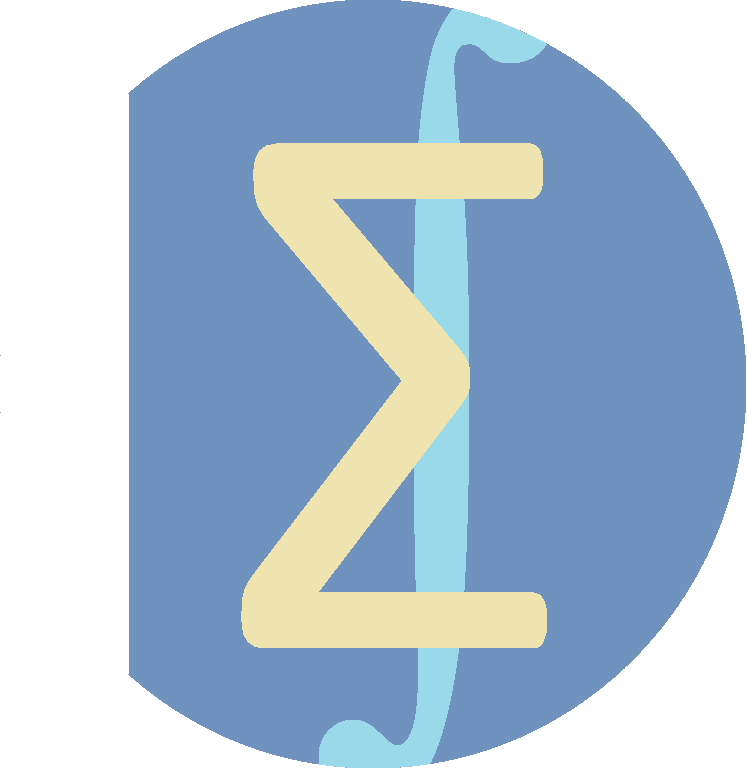
\includegraphics[width=1cm]{logo}
            
        \Large
        www.statmania.info\\
            
    \end{center}
\end{titlepage}


\begin{questions}

\section{Basic Concept of Statistics}

\question \textbf{Who is known as the Father of modern statistics?}
\choice{P.C. Mahalanobis}{Kazi Motaher Hossain}{Karl Pearson}{R.A. Fisher}{d}

\question \textbf{If $\displaystyle \sum_{i=1}^{20} x_i^2=20$ and $\displaystyle \sum_{i=1}^{20} x_i=30$, what is the value of $\displaystyle \sum_{i=1}^{20} x_i^2 + \sum_{i=1}^{20} x_i + 100$?}
\choice{130}{200}{230}{2130}{c}

\question \textbf{A subset of a population is called--}
\choice{Constant}{Variable}{Sample}{Scale}{c}

\question \textbf{How many measurement scales are there?}
\choice{2}{3}{4}{5}{c}

\question \textbf{Which of the following is a continuous variable?}
\choice{Number of goals}{Natural number}{Summation of Fibonacci series}{Success rate}{d}

\question \textbf{In which scale of measurement, zero is regarded as true zero?}
\choice{Nominal scale}{Interval scale}{Ratio scale}{Ordinal scale}{c}

\question \textbf{Which is a discrete variable?}
\choice{Weight}{Amount of rainfall}{Distance}{Grade in a subject}{d}

\question \textbf{$If x_1=2, x_2=-3, x_3=7$, and $x_4=12, \displaystyle \sum_{i=1}^4 x_i^2=?$}
\choice{26}{106}{206}{216}{c}

\question \textbf{Which one falls in the category of interval scale?}
\choice {Temperature}{Speed}{Distance}{Film rating}{a}

\question \textbf{In which scale of measurement, zero is regarded as true zero?}
\choice{Nominal scale}{Interval scale}{Ratio scale}{Ordinal scale}{c}

\question \textbf{Which is a discrete variable?}
\choice{Weight}{Amount of rainfall}{Distance}{Grade in a subject}{d}

\question \textbf{Which one is product of square?}
\choice {$\prod x_i^2$}{$(\prod x_i)^2$}{$\sum x_i^2 \times \sum x$}{$\sum x_i^2$}{a}

\question \textbf{For which variable, determining number of terms is not possible?}
\choice{Discrete variable}{Continuous variable}{Quantitative variable}{Qualitative variable}{b}

\textbf{Answer the next three question based on the following information.}

\textbf{A farmer collects growth (in cm) of 10 plants in a month and finds that \\ $\sum x_i = 7$ and $\sum x_i^2=15$}

\question \textbf{What is the value of $\sum (x_i+4)$?}
\choice{23}{$\sum x_i +4n$}{22}{11}{a}

\question \textbf{What is the value of $\sum (x_i-4)^2$?}
\choice{23}{135}{484}{121}{a}

\question \textbf{If the square of summation is subtracted the sum of square, the value is - }
\choice{-8}{34}{8}{-34}{d}

\question \textbf{Which one is not an example of ratio scale?}
\choice{Room no.}{Income}{Number of accidents}{Weight}{a}

\section{Collection, Organization, and Presentation of Data}

\question \textbf{How many sources of data are there?}
\choice{5}{4}{3}{2}{d}

\question \textbf{Data obtained through direct observation is called--}
\choice{Primary data}{Secondary data}{Original Data}{Informal data}{a}

\question \textbf{Who invented Stem and Leaf plot?}
\choice{Karl Pearson}{R.A. Fisher}{David Cox}{John Tukey}{d}

\question \textbf{Which rule is suggested by H.G. Sturges for determining number of class (k)?}
\choice{$K=1+3.322logN$}{$K=1+3.222logN$}{$K=1-3.222logN$}{$K=1+2.332logN$}{a}

\question \textbf{To show runs per over in a cricket match, which diagram can be used?}
\choice{Histogram}{Bar Diagram}{Ogive}{Frequency polygon}{b}

\section{Measures of Central Tendency}

\subsection{General Questions}

\question \textbf{How many measure of central tendency are there?}
\choice{2}{3}{4}{5}{d}

\question \textbf{Which measure of central tendencyis suitable for qualitative variable?}
\choice{Arithmetic Mean}{Harmonic Mean}{Quadratic Mean}{Mode}{d}

\question \textbf{In presence of negative values, which measure is not usable?}
\choice{Arithmetic Mean}{Geometric Mean}{Quadratic Mean}{Harmonic Mean}{b}

\question \textbf{Inappropriate for algebraic analysis--}

i. Median \\
ii. Mode \\
iii. Geometric Mean

Which one is true?

\choice{i}{ii}{i \& ii}{ii \& iii}{c}

\textbf{Answer the next two questions based on the following information}

  \begin{table}[h]
\centering
\begin{tabular}{cccccc}
Accident     & 4 & 6 & 7 & 8 & 9\\ \hline
Frequency & 2   & 0    & 4     & 4     & 1   
\end{tabular}
\end{table}
\question \textbf{Fifth Decile is --}
\choice{0}{8}{7}{6}{c}

\question \textbf{Which of the following is mode?}
\choice{4}{8}{0}{7}{b}

\question \textbf{Which measure gives a value from within the values?}
\choice{Arithmetic Mean}{Geometric Mean}{Median}{Mode}{d}

\question \textbf{Which one is not a proper measure of central tendency?}
\choice{2nd Quartile}{Third Decile}{3rd Quintile}{110th Percentile}{d}

\question \textbf{Which measure is not used in determining skewness?}
\choice{Arithmetic Mean}{Geometric Mean}{Median}{Mode}{b}

\question \textbf{When is the relationship $AM = HM = GM$ true?}
\choice {All values are equal}{The values form a geometric progression}{ The values form an arithmetic progression}{All values are distinct}{a}

\question \textbf{In the presence of outlier(s), which measure of central tendency is suitable?}
\choice {Arithmetic mean}{Median}{Quadratic mean}{Power mean}{b}

\question \textbf{If a rate is defined as $R = \frac cd$, where c is constant, then which measure is perfect?}
\choice {Weighted arithmetic mean}{Harmonic mean}{Quadratic mean}{Weighted geometric mean}{b}

\question \textbf{Which measure might have more than one value?}
\choice{Arithmetic mean}{Geometric mean}{Quadratic mean}{Mode}{d}

\subsection{Arithmetic Mean}

\question \textbf{For grouped data, which formula is correct for Arithmetic Mean?}
\choice{$\displaystyle \bar x = \frac{\sum f_ix_i}{\sum f_i}$}{$\displaystyle \bar x = \frac{\sum x_i}{N}$}{$\displaystyle \bar x = \frac{\sum f_ix_i}{n}$}{$ \displaystyle\bar x = \frac{\sum f_i}{N}$}{a}

\question \textbf{Arithmetic mean of the series 2, 12, 22, $\cdots$, 92 is--}
\choice{45}{46}{47}{55}{c}

\question \textbf{What is the arithmetic mean of first n odd natural numbers?}
\choice{$\frac{n+1}{n}$}{n}{n+1}{$\frac{n+1}{2}$}{b}

\question \textbf{What is the arithmetic mean of first n even natural numbers?}
\choice{$\frac{n+1}{2}$}{$n+1$}{$n$}{$\frac{n-1}{2}$}{b}

\question \textbf{The arithmetic mean of first n natural numbers-}
\choice {$\frac{n}{2}$}{$\frac{n+1}{2}$}{$\frac{n^2}{2}$}{$\frac{n^2-1}{2}$}{b}

\question \textbf{Arithmetic means of three groups having equal no. of items are 30, 32, and 34. What is the combined mean?}
\choice{30.33}{32.67}{32.00}{33.00}{c}

\subsection{Median}

\question \textbf{Median can be determined from the--}
\choice{Histogram}{Frequency curve}{Ogive}{Pie Chart}{c}

\textbf{Answer the next two (2) questions based on the following information}

\begin{table}[h]
\centering
\begin{tabular}{c|c|c|c|c|c|c}
Class                                                           & $\le 20$ & 20-25 & 25-50 & 50-60 & 69-70 & $\ge 70$ \\ \hline
Frequency                                                       & 5        & 10    & 10    & 7     & 5     & 3        \\ \hline
\begin{tabular}[c]{@{}c@{}}Cumulative \\ Frequency\end{tabular} & 5        & 15    & 25    & 32    & 37    & 40      
\end{tabular}
\end{table}

\question \textbf{How many values are between 20 and 70?}
\choice{20}{32}{35}{37}{b}

\question \textbf{Which one is the median class?}
\choice{20-25}{25-50}{50-60}{60-70}{b}

\subsection{Partition Values}

\textbf{Answer the next two questions as per the following information.}

42 44 59 64 70 72 74 91 94 are 9 values.

\question \textbf{What is the 50th percentile?}
\choice {64}{70}{72}{71}{b}

\question \textbf{Below which value lie 70 percent values?}
\choice {42}{44}{59}{74}{d}

\question \textbf{Above which value lie 30\% observations?}
\choice{3rd Quartile}{Median}{30th Percentile}{70th percentile}{d}



\section{Measures of Dispersion}

\question \textbf{Which of the following is the best measure of dispersion?}
\choice{Range}{Mean deviation}{Standard deviation}{Coefficient of variation}{c}

\question \textbf{What is the minimum possible value of standard deviation?}
\choice{$\infty$}{-1}{0}{1}{c}

\question \textbf{For two values, range is found to be 8. What are the values of mean deviation and standard deviation}
\choice{(2,4)}{(4,4)}{(4,8)}{(8,8)}{a}

\question \textbf{What is the standard deviation of first 10 natural numbers?}
\choice{2.87}{3.02}{0}{2.78}{a}

\question \textbf{Which measure is unit-free?}
\choice{Range}{Mean deviation}{Standard deviation}{Coefficient of variation}{d}

\section{Moments, Skewness, and Kurtosis}

\subsection{Moments}

\question \textbf{Which can be used to measure dispersion?}
\choice{$\mu_2'$}{$\mu_1$}{$\mu_2$}{$\mu_1'$}{c}

\question \textbf{The formula of coefficient of variance (CV) is --}
\choice{$\frac{\mu_2}{n}\times 100$}{$\frac{\mu_2}{\mu_1}\times 100$}{$\frac{\mu_2}{\bar x}\times 100$}{$\frac{\mu_3}{\sigma}\times 100$}{c}

\question \textbf{First moment around zero is --}
\choice{0}{1}{-1}{Arithmetic Mean}{d}

\question \textbf{Which might have a negative value?}
\choice{$\mu_4$}{$\mu_3$}{$\mu_2'$}{$\mu_2$}{b}

\question \textbf{2nd Central Moment is --}
\choice{$\mu_2-\mu_1'$}{$\mu_2+\mu_1'$}{$\mu_2-\mu_1'^2$}{$\mu_2'-\mu_1'^2$}{d}

\question \textbf{First central moment is equal to --}
\choice{1}{0}{-1}{$\bar x-a$}{b}

\question \textbf{First moment around a is equal to --}
\choice{1}{0}{-1}{$\bar x-a$}{d}

\question \textbf{The first raw moment about 3 is -5. What is the value of arithmetic mean?}
\choice{2}{-2}{0}{8}{b}

\question \textbf{Moments can be--}

i. positive \\
ii. not negative \\
iii. positive or negative

\textbf{Which one is correct?}

\choice{i and ii}{i and iii}{ii and iii}{i, ii and iii}{b}

\subsection{Skewness}

\question \textbf{For a data, $Q_3=41.6, Q_1=17.2, Median = 29, \& AM = 30$; What is Coefficient of skewness?}
\choice{24.4}{1}{0.03}{29.45}{d}

\question \textbf{In case of positive skewness, which one is correct?}
\choice{$Mean>Median>Mode$}{$Mean<Median<Mode$}{$Mean=Median=Mode$}{$Mean>Median<Mode$}{a}

\question \textbf{For a symmetrical distribution, $\beta_1=$}
\choice{1}{-1}{0}{3}{c}

\question \textbf{$\sqrt{\beta_1}=-0.23$ implies--}
\choice{Left Skew}{Symmetry}{Right Skew}{Mesokurtic}{a}

\subsection{Kurtosis}

\question \textbf{The standard deviation of a mesokurtik distribution is 2. What is the value of the 4th central moment?}
\choice{4}{8}{16}{48}{d}

\question \textbf{$\beta_2 = \sqrt 9$ implies data are--}
\choice{Leptokurtic}{Platykurtic}{Mesokurtic}{Symmetric}{c}

\question \textbf{For a mesokurtik distribution, $\beta_2 = --$}
\choice{0}{-3}{3}{1}{c}

\subsection{Misc}

\question \textbf{Which is not used in constructing Box \& Whisker Plot?}
\choice{Mode}{$X_L$}{$Q_1 \& Q_3$}{$Q_1, Q_2 \& Q_3$}{a}

\question \textbf{In a symmatric distribution--}

i. Arithmetic Mean = Mode = Median \\
ii. $Q_2-Q_1 = Q_3-Q_2$  \\
iii. $Q_1-X_L = X_H-Q_3$

Which one is true?

\choice{i \& ii}{ii \& iii}{i \&iii}{i, ii \&iii}{d}

\question \textbf{Which is not included in five number summary?}
\choice{Arithmetic Mean}{$X_H$}{$Q_2$}{$Q_3$}{a}

\section{Correlation and Regression}

\section{Time Series}

\question \textbf{A company is constantly getting greater revenue than previous year; this is--}
\choice{Seasonal Variation}{General Trend}{Irregular Variation}{Cyclic Variation}{b}

\question \textbf{Which is not a method of finding general trend?}
\choice{Graphical Method}{Moving Average}{Semi-Average}{Moving Median}{d}

\textbf{Answer the next two questions based on the following table:}

  \begin{table}[h]
\centering
\begin{tabular}{ccccccc}
Year     & 2007 & 2008 & 2009 & 2010 & 2011 & 2012\\ \hline
Sales & 5   & 35    & 34     & 40     & 42  & 204 
\end{tabular}
\end{table}

\question \textbf{In Semi-Average method, what is the 2nd average?}
\choice{74}{24.67}{95.33}{28}{c}

\question \textbf{For this data, which method would give the best measure of trend?}
\choice{3-yearly Moving Average}{4-yearly Moving Average}{Semi-Average}{Graphical Method}{a}

\question \textbf{which component of time series represents a natural disaster?}
\choice{Seasonal Variation}{General Trend}{Irregular Variation}{Cyclic Variation}{c}

\section{Published Statistics in Bangladesh}

\question \textbf{Bangladesh Bureau of Statistics collect -- }
\choice{Official statistics}{Non-official statistics}{Semi-official statistics}{None of the above}{a}

\question \textbf{Which statistics are published by an NGO?}
\choice{Official statistics}{Non-official statistics}{Semi-official statistics}{None of the above}{c}

\question \textbf{The primary source of official statistics in Bangladesh is --}
\choice{WHO}{BBS}{CPD}{UNDP}{b}

\question \textbf{In Bangladesh, a census is usually done every -- years}
\choice{20}{15}{10}{12}{c}

%\question \textbf{To complete the song, the last answer should be
%\choice{a}{b}{c}{d}{e} % Invalid answer choice

\end{questions}

\newpage  %Uncomment to put on new age
\bigskip

\begin{multicols}{4}
[
Answer Key: 
]
\showallanswers % Phil Hirschorn
\end{multicols}


\end{document}